\section{Proposed Methodology}

In this section, we describe our pipeline that consists of preprocessing, optical flow estimation, feature extraction, temporal sequence modeling with BiLSTM+Attention, training procedure, and interpretability module. The implementation details are outlined in Algorithm~\ref{alg:pipeline}.

\subsection{Overall Pipeline}

The proposed system accepts a raw video stream as input and produces a frame-level binary classification: \textit{stampede} or \textit{normal}. The processing pipeline consists of six sequential stages:

\begin{enumerate}
  \item \textbf{Preprocessing:} Each frame is converted to grayscale, resized to a fixed resolution, and smoothed with a Gaussian filter.
  \item \textbf{Dense optical flow:} The Farneb\"{a}ck algorithm is applied between consecutive preprocessed frames to produce a per-pixel displacement field.
  \item \textbf{Feature extraction:} Nine scalar statistics are computed from each displacement field within a sliding temporal window.
  \item \textbf{Sequence construction:} Feature vectors from consecutive windows are grouped into overlapping temporal sequences and standardised.
  \item \textbf{Classification:} A BiLSTM+Attention network processes each sequence and outputs a stampede probability.
  \item \textbf{Explainability (optional):} Permutation feature importance and attention-weight visualisation are invoked to inspect the model's reasoning.
\end{enumerate}

Figure~\ref{fig:pipeline} illustrates the end-to-end architecture.

\begin{center}
  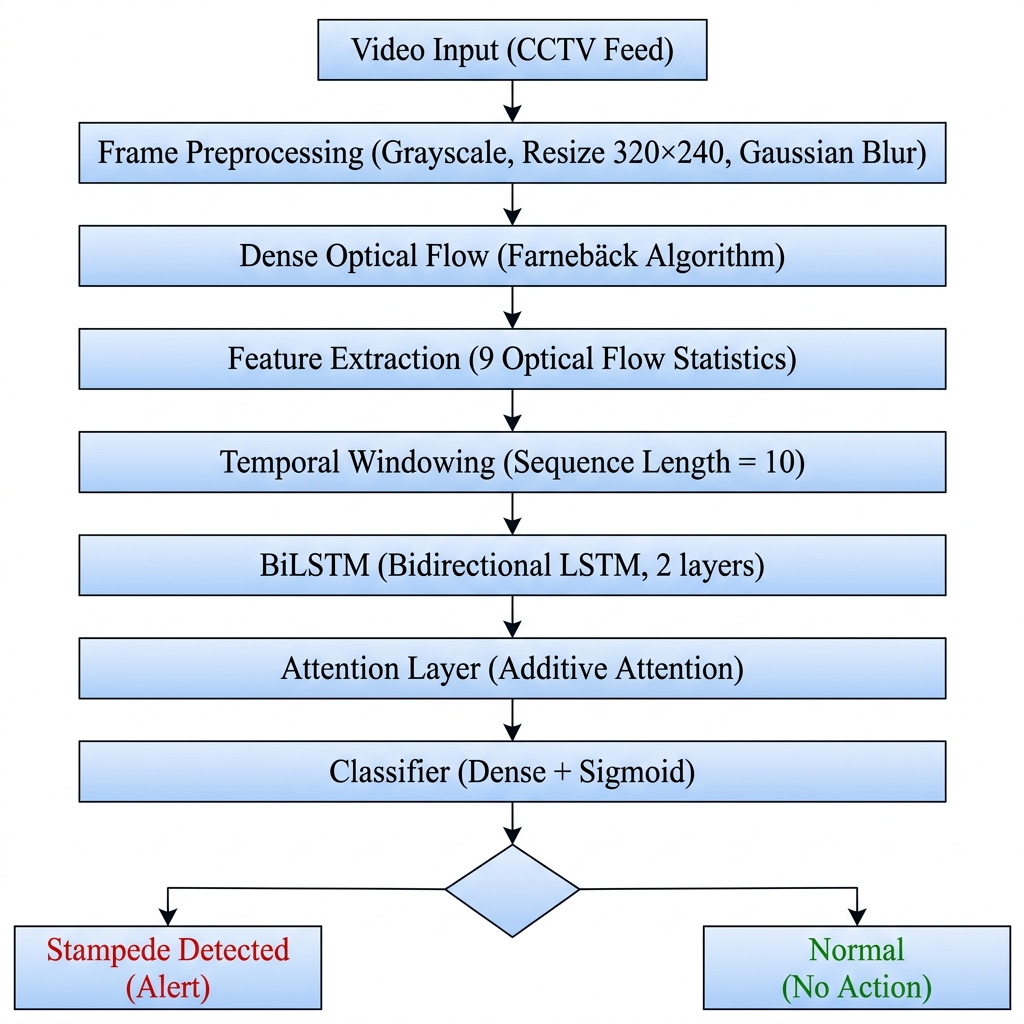
\includegraphics[width=0.85\linewidth]{figures/pipeline_flowchart.png}
  \captionof{figure}{End-to-end pipeline of the proposed stampede detection system. Raw video frames pass through preprocessing, optical flow computation, nine-feature extraction, temporal sequencing, BiLSTM+Attention classification, and optional explainability analysis.}
  \label{fig:pipeline}
\end{center}

\begin{table}[H]
\centering
\caption{Algorithm 1: End-to-end stampede detection pipeline.}
\label{alg:pipeline}
\footnotesize
\begin{tabular}{p{0.92\linewidth}}
\toprule
\textbf{Algorithm 1:} Stampede Detection Pipeline \\
\midrule
\textbf{Input:} Video stream $\mathcal{V} = \{I_1, I_2, \ldots, I_T\}$ \\
\textbf{Output:} Per-sequence label $\hat{y} \in \{0, 1\}$ and attention weights $[\alpha_1, \ldots, \alpha_S]$ \\
\midrule
1: \textbf{for} each frame $I_t$ in $\mathcal{V}$ \textbf{do} \\
2: \quad Convert $I_t$ to 8-bit grayscale: $G_t \leftarrow \text{rgb2gray}(I_t)$ \\
3: \quad Resize: $G_t \leftarrow \text{resize}(G_t, 320 \times 240)$ \\
4: \quad Smooth: $G_t \leftarrow \text{GaussianBlur}(G_t, k{=}5)$ \\
5: \textbf{end for} \\
6: \textbf{for} each consecutive pair $(G_t, G_{t+1})$ \textbf{do} \\
7: \quad Compute dense optical flow: $(d_x, d_y) \leftarrow \text{Farneb\"{a}ck}(G_t, G_{t+1})$ \\
8: \quad Convert to polar: $M_t \leftarrow \sqrt{d_x^2 + d_y^2}$, \; $\theta_t \leftarrow \arctan(d_y / d_x)$ \\
9: \textbf{end for} \\
10: \textbf{for} each sliding window $w$ of $L{=}15$ consecutive flow frames \textbf{do} \\
11: \quad Extract 9 features: $\mathbf{v}_w \leftarrow [H, \text{TOV}, \text{KDE}, \bar{M}, \sigma_M, \gamma_M, C, \rho, \sigma^2_\theta]$ \\
12: \textbf{end for} \\
13: Group feature vectors into sequences: $\mathbf{X}_i = \{\mathbf{v}_{w}, \ldots, \mathbf{v}_{w+S-1}\}$, $S{=}10$ \\
14: Standardise features: $\mathbf{X}_i \leftarrow (\mathbf{X}_i - \boldsymbol{\mu}_\text{train}) / \boldsymbol{\sigma}_\text{train}$ \\
15: \textbf{for} each sequence $\mathbf{X}_i$ \textbf{do} \\
16: \quad Forward pass through BiLSTM+Attention: $\hat{y}_i, [\alpha_1, \ldots, \alpha_S] \leftarrow f_\Theta(\mathbf{X}_i)$ \\
17: \quad Classify: label $\leftarrow \mathbf{1}[\hat{y}_i > 0.5]$ \\
18: \textbf{end for} \\
19: \textbf{return} labels and attention weights \\
\bottomrule
\end{tabular}
\end{table}

\subsection{Preprocessing}

Each video frame $I_t$ undergoes three preprocessing steps before optical flow computation. First, the frame is converted from RGB to 8-bit grayscale, since the Farneb\"{a}ck algorithm operates on single-channel luminance values and colour information does not contribute to displacement estimation. Second, the grayscale frame is resized to a fixed resolution of $320 \times 240$ pixels using bilinear interpolation. This standardisation ensures that the pipeline processes videos from cameras with different native resolutions in a consistent manner and that the downstream feature statistics are comparable across scenes. Third, a $5 \times 5$ Gaussian blur with $\sigma = 1.1$ is applied to attenuate high-frequency sensor noise that would otherwise produce spurious flow vectors. No data augmentation or additional preprocessing is performed during inference.

\subsection{Optical Flow Computation}

Dense optical flow is computed between every pair of consecutive preprocessed frames using the Farneb\"{a}ck algorithm \cite{farneback2003two}. This algorithm approximates the local neighbourhood of each pixel $\mathbf{x} = (x, y)$ as a quadratic polynomial:

\begin{equation}
  f(\mathbf{x}) \approx \mathbf{x}^T A \mathbf{x} + \mathbf{b}^T \mathbf{x} + c
  \label{eq:polynomial}
\end{equation}

\noindent where $A \in \mathbb{R}^{2 \times 2}$ is a symmetric matrix encoding the local curvature, $\mathbf{b} \in \mathbb{R}^2$ is a gradient vector, and $c \in \mathbb{R}$ is a scalar offset. All three quantities are estimated through a weighted least-squares fit using a Gaussian weighting kernel centred on $\mathbf{x}$. When the same spatial region is observed in the subsequent frame, the polynomial coefficients shift. The displacement vector $\mathbf{d} = (d_x, d_y)$ that best explains the coefficient change is solved for analytically, yielding a dense flow field over the entire frame.

The Cartesian displacement field is converted to polar coordinates to obtain a magnitude map $M(x,y)$ and a direction map $\theta(x,y)$:

\begin{equation}
  M(x,y) = \sqrt{d_x^2 + d_y^2}, \qquad \theta(x,y) = \arctan\!\left(\frac{d_y}{d_x}\right)
  \label{eq:polar}
\end{equation}

For each pair of consecutive frames, two $320 \times 240$ matrices are thus produced: $M$, which quantifies the speed of motion at each pixel, and $\theta$, which encodes the direction of motion. The Farneb\"{a}ck algorithm is configured with 5 pyramid levels, a pyramid scale of 0.5, a window size of 15, 3 iterations per level, and a polynomial neighbourhood size of 5---values chosen to balance accuracy against computational cost for the target frame resolution.

\subsection{Feature Extraction}

A sliding window of $L = 15$ consecutive flow frames is advanced across the video with a stride of 1 frame. Within each window, nine scalar statistics are computed from the pooled magnitude and direction maps to form a feature vector $\mathbf{v} \in \mathbb{R}^9$. Three features are adopted from prior work \cite{cobparro2021stampede}; six are newly proposed. Table~\ref{tab:features} summarises all nine features along with their physical interpretation.

\begin{table*}[!t]
\centering
\caption{The nine optical-flow features computed per temporal window. Features 1--3 are adopted from prior work; features 4--9 are proposed in this study.}
\label{tab:features}
\footnotesize
\begin{tabular}{clcl}
\toprule
\textbf{\#} & \textbf{Feature Name} & \textbf{Source} & \textbf{Physical Interpretation} \\
\midrule
1 & Entropy ($H$)         & Prior work & Disorder in movement directions \\
2 & TOV                    & Prior work & Frame-to-frame change in active motion region \\
3 & KDE                    & Prior work & Kernel density estimate of flow magnitudes \\
4 & Mean Magnitude ($\bar{M}$) & \textbf{Proposed} & Average crowd speed \\
5 & Std. Magnitude ($\sigma_M$) & \textbf{Proposed} & Speed variability among individuals \\
6 & Skewness ($\gamma_M$)  & \textbf{Proposed} & Asymmetry of speed distribution \\
7 & Motion Coherence ($C$) & \textbf{Proposed} & Fraction of crowd moving in a shared direction \\
8 & Crowd Density ($\rho$) & \textbf{Proposed} & Fraction of pixels with active motion \\
9 & Direction Variance ($\sigma^2_\theta$) & \textbf{Proposed} & Angular scatter of motion vectors \\
\bottomrule
\end{tabular}
\end{table*}

The mathematical definitions of all nine features are provided below. Let $\mathcal{P} = \{(x,y) : M(x,y) > \tau\}$ denote the set of \textit{active pixels} whose flow magnitude exceeds a minimum threshold $\tau = 0.5$ pixels/frame, and let $N = |\mathcal{P}|$ be the count of active pixels.

\subsubsection{Adopted Features}

\textbf{Entropy ($H$).} The flow direction histogram is constructed by quantising the angle $\theta$ into $B = 8$ bins of $45^\circ$ each. Letting $p_b$ denote the fraction of active pixels falling in bin $b$, the Shannon entropy is:

\begin{equation}
  H = -\sum_{b=1}^{B} p_b \log_2 p_b
  \label{eq:entropy}
\end{equation}

$H$ is low when most people move in a shared direction (few bins dominate) and high when movement directions are uniformly distributed (all bins equally populated), as occurs during panic scatter.

\textbf{Temporal Occupancy Variation (TOV).} TOV measures the frame-to-frame change in the spatial extent of the active motion region. Let $O_t$ denote the set of active pixels at time $t$. TOV is defined as:

\begin{equation}
  \text{TOV} = \frac{1}{L-1} \sum_{t=1}^{L-1} \frac{|O_{t+1} \triangle O_t|}{W \times H_{\text{img}}}
  \label{eq:tov}
\end{equation}

\noindent where $\triangle$ denotes the symmetric difference and $W \times H_{\text{img}}$ is the frame area. TOV captures the spatial spread of panic: a rapid expansion of the motion region indicates that disturbance is propagating outward through the crowd.

\textbf{Kernel Density Estimation (KDE).} The probability density function of the flow magnitude is estimated with a Gaussian kernel density estimator, and KDE is determined by finding the maximum point of the distribution. Peaks of the KDE illustrate the values of the flow magnitude that contribute the most to the probability density function. When a crowd moves with consistent speed, the density function will peak at a certain point, whereas an abnormal flow will involve varied speeds.

\subsubsection{Proposed Features}

\textbf{Mean Magnitude ($\bar{M}$).} The average of the flow magnitude over all pixels is used as a metric of the mean crowd speed in a given frame.

\begin{equation}
  \bar{M} = \frac{1}{N} \sum_{i \in \mathcal{P}} M_i
  \label{eq:mean_mag}
\end{equation}

\textbf{Standard Deviation of Magnitude ($\sigma_M$).} The standard deviation of the magnitude characterizes the spread of the speed distribution.

\begin{equation}
  \sigma_M = \sqrt{\frac{1}{N} \sum_{i \in \mathcal{P}} (M_i - \bar{M})^2}
  \label{eq:std_mag}
\end{equation}

During anomalous events, the standard deviation of the flow magnitude typically increases due to the presence of both fast and slow-moving crowds.

\textbf{Skewness ($\gamma_M$).} The third standardised moment of the magnitude distribution captures distributional asymmetry:

\begin{equation}
  \gamma_M = \frac{1}{N} \sum_{i \in \mathcal{P}} \left(\frac{M_i - \bar{M}}{\sigma_M}\right)^3
  \label{eq:skewness}
\end{equation}

Positive skewness indicates a right-tailed distribution (a few individuals moving much faster than the crowd average), which is characteristic of early-stage panic where only a subset of the crowd has begun to flee.

\textbf{Motion Coherence ($C$).} Motion coherence measures the fraction of active pixels whose flow direction falls within one standard deviation of the dominant (mean) direction:

\begin{equation}
  C = \frac{1}{N} \sum_{i \in \mathcal{P}} \mathbf{1}\!\left[|\theta_i - \bar{\theta}| < \sigma_\theta\right]
  \label{eq:coherence}
\end{equation}

\noindent where $\bar{\theta}$ is the circular mean of the flow angles and $\sigma_\theta$ is the circular standard deviation. $C$ approaches 1.0 when the crowd moves cohesively and drops toward 0 during multidirectional scatter.

\textbf{Crowd Density ($\rho$).} Crowd density is defined as the fraction of total pixels that exhibit active motion:

\begin{equation}
  \rho = \frac{N}{W \times H_{\text{img}}}
  \label{eq:density}
\end{equation}

This feature captures the spatial extent of crowd activity. During a stampede, $\rho$ typically increases as previously stationary individuals begin to move.

\textbf{Direction Variance ($\sigma^2_\theta$).} Direction variance is computed as the circular variance of flow angles across all active pixels:

\begin{equation}
  \sigma^2_\theta = 1 - \left| \frac{1}{N} \sum_{i=1}^{N} e^{j\theta_i} \right|
  \label{eq:dir_var}
\end{equation}

\noindent where $j = \sqrt{-1}$. This formulation maps the unit-circle representation of angles to a scalar in $[0, 1]$: $\sigma^2_\theta \approx 0$ when all flow vectors point in a common direction, and $\sigma^2_\theta \to 1$ when directions are uniformly distributed. Empirically, direction variance emerged as the single most discriminative feature in the ablation study (Section~5.2), consistent with the intuition that multidirectional scatter is the defining kinematic signature of a crowd crush.

\subsection{Temporal Sequence Construction}

The per-window feature vectors are grouped into overlapping temporal sequences of length $S = 10$ windows, with a stride of 1 window. At 30~FPS with $L = 15$ frames per window, each sequence spans approximately 5 seconds of video. A sequence is assigned the anomalous label ($y = 1$) if any of its constituent windows falls within the annotated stampede phase; otherwise it is labelled as normal ($y = 0$).

Before being passed to the classifier, all features are standardised using $z$-score normalisation:

\begin{equation}
  \hat{v}^{(j)} = \frac{v^{(j)} - \mu_{\text{train}}^{(j)}}{\sigma_{\text{train}}^{(j)}}
  \label{eq:zscore}
\end{equation}

\noindent where $\mu_{\text{train}}^{(j)}$ and $\sigma_{\text{train}}^{(j)}$ are the mean and standard deviation of feature $j$ computed on the training split. This normalisation ensures that features with naturally larger magnitudes (e.g., mean flow speed) do not dominate those with smaller scales (e.g., skewness) during gradient-based optimisation.

\subsection{BiLSTM + Attention Architecture}

\begin{center}
  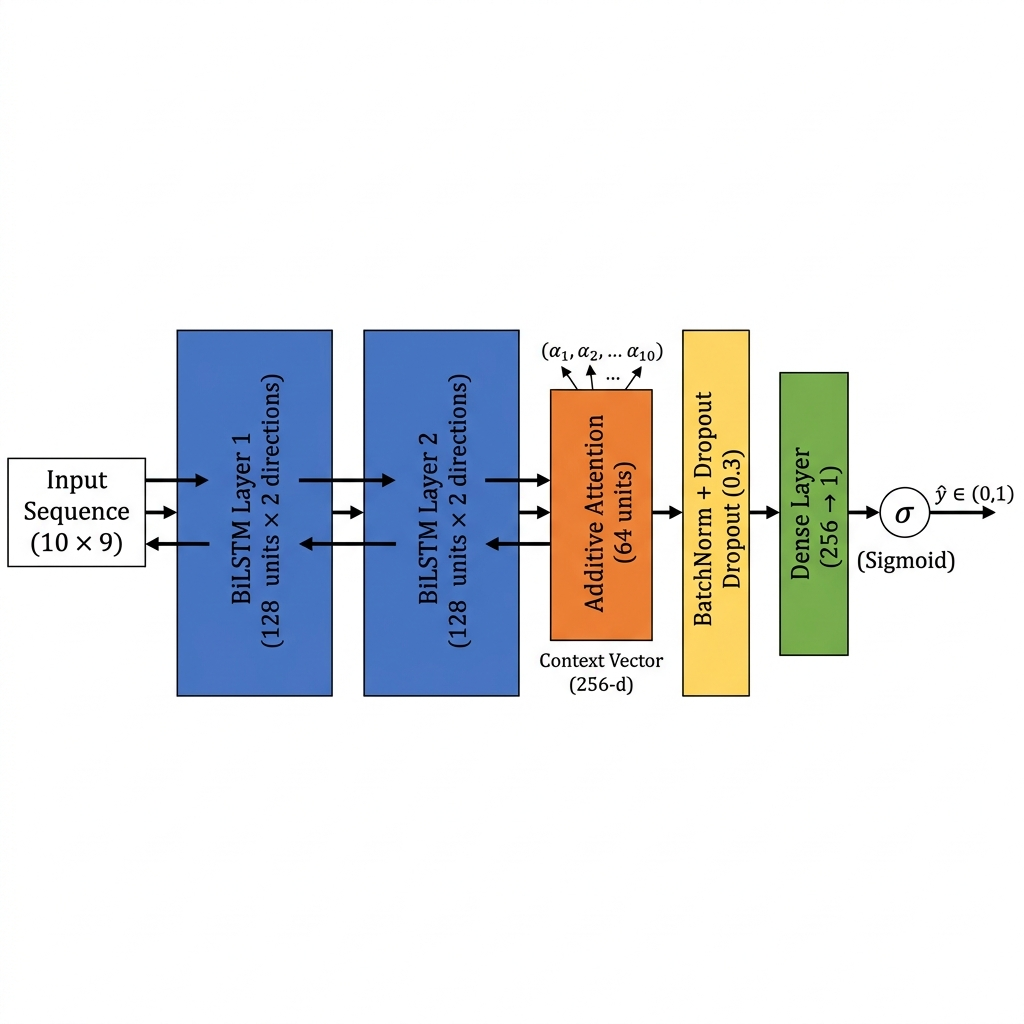
\includegraphics[width=0.85\linewidth]{figures/model_architecture.png}
  \captionof{figure}{Architecture of the proposed BiLSTM+Attention classifier. The input sequence passes through a two-layer Bidirectional LSTM, followed by an additive attention layer, Batch Normalisation, Dropout, and a sigmoid output unit.}
  \label{fig:architecture}
\end{center}

The classifier consists of three components: a Bidirectional LSTM encoder, an additive attention layer, and a classification head.

\subsubsection{Bidirectional LSTM Encoder}
A two-layer Bidirectional LSTM \cite{chung2014bilstm} with 128 hidden units per direction processes the input sequence $\mathbf{X} = \{x_1, \ldots, x_S\}$, where each $x_t \in \mathbb{R}^9$. The forward LSTM reads the sequence from $t = 1$ to $t = S$, producing hidden states $\overrightarrow{\mathbf{h}}_t$. A second LSTM reads the sequence in reverse, from $t = S$ to $t = 1$, producing $\overleftarrow{\mathbf{h}}_t$. The two are concatenated at each time-step:

\begin{equation}
  \mathbf{h}_t = \left[\overrightarrow{\mathbf{h}}_t \;\|\; \overleftarrow{\mathbf{h}}_t\right], \quad \mathbf{h}_t \in \mathbb{R}^{256}
  \label{eq:bilstm}
\end{equation}

Each hidden state $\mathbf{h}_t$ thus encodes temporal context from both preceding and subsequent frames within the analysis window. This is particularly valuable for stampede detection, as the ambiguous frames immediately preceding a panic onset become more interpretable when information about the subsequent escalation is available.

\subsubsection{Additive Attention Layer}
An additive (Bahdanau-style) attention mechanism \cite{bahdanau2015neural} is applied over the BiLSTM hidden states. A learned scoring function assigns an importance weight to each time-step:

\begin{equation}
  e_t = \mathbf{v}^T \tanh\!\left(W_a \mathbf{h}_t + \mathbf{b}_a\right)
  \label{eq:attn_score}
\end{equation}

\noindent where $W_a \in \mathbb{R}^{d_a \times 256}$ is a weight matrix, $\mathbf{b}_a \in \mathbb{R}^{d_a}$ is a bias vector, and $\mathbf{v} \in \mathbb{R}^{d_a}$ is a learned context vector, with $d_a = 128$. The raw scores are normalised via softmax to produce attention weights:

\begin{equation}
  \alpha_t = \frac{\exp(e_t)}{\sum_{k=1}^{S} \exp(e_k)}, \quad \sum_{t=1}^{S} \alpha_t = 1
  \label{eq:attn_weights}
\end{equation}

The final context vector is computed as a weighted sum of the hidden states:

\begin{equation}
  \mathbf{c} = \sum_{t=1}^{S} \alpha_t \mathbf{h}_t, \quad \mathbf{c} \in \mathbb{R}^{256}
  \label{eq:context}
\end{equation}

Unlike fixed pooling strategies (e.g., taking the last hidden state or averaging all states), this mechanism allows the model to concentrate on the specific time-steps where abnormal motion patterns emerge, assigning near-zero weights to windows that contain only normal crowd behaviour.

\subsubsection{Classification Head}
The context vector $\mathbf{c}$ is passed through a Batch Normalisation layer for training stability, followed by Dropout with rate $p = 0.3$ for regularisation, and finally a fully connected layer with a single output unit and sigmoid activation:

\begin{equation}
  \hat{y} = \sigma\!\left(\mathbf{w}^T \text{Dropout}\!\left(\text{BN}(\mathbf{c})\right) + b\right)
  \label{eq:output}
\end{equation}

\noindent where $\sigma(\cdot)$ denotes the sigmoid function. The output $\hat{y} \in (0, 1)$ represents the estimated probability that the input sequence contains a stampede event. The complete model has 554,817 trainable parameters.

\subsection{Training Procedure}

The model is trained by minimising the Binary Cross-Entropy loss with logits:

\begin{equation}
  \mathcal{L} = -\frac{1}{N_{\text{batch}}} \sum_{i=1}^{N_{\text{batch}}} \left[ y_i \log(\hat{y}_i) + (1 - y_i) \log(1 - \hat{y}_i) \right]
  \label{eq:bce}
\end{equation}

\noindent where $y_i \in \{0, 1\}$ is the ground-truth label and $\hat{y}_i$ is the predicted probability for the $i$-th sequence. The Adam optimiser is used with an initial learning rate of $10^{-3}$, $\beta_1 = 0.9$, and $\beta_2 = 0.999$. If the validation loss does not improve for 5 consecutive epochs, the learning rate is halved using a ReduceLROnPlateau scheduler. Training proceeds for up to 100 epochs with an early stopping patience of 15 epochs based on validation loss. The batch size is 32. Algorithm~\ref{alg:training} summarises the training procedure.

\begin{table}[H]
\centering
\caption{Algorithm 2: BiLSTM+Attention training procedure.}
\label{alg:training}
\footnotesize
\begin{tabular}{p{0.92\linewidth}}
\toprule
\textbf{Algorithm 2:} Model Training \\
\midrule
\textbf{Input:} Training sequences $\{(\mathbf{X}_i, y_i)\}_{i=1}^{N_\text{train}}$, validation set $\mathcal{D}_\text{val}$ \\
\textbf{Output:} Trained parameters $\Theta^*$ \\
\midrule
1: Initialise model parameters $\Theta$ \\
2: Set $\text{lr} \leftarrow 10^{-3}$, $\text{patience}_\text{lr} \leftarrow 5$, $\text{patience}_\text{stop} \leftarrow 15$ \\
3: Set $\text{best\_loss} \leftarrow \infty$, $\text{wait} \leftarrow 0$ \\
4: \textbf{for} epoch $= 1, 2, \ldots, 100$ \textbf{do} \\
5: \quad \textbf{for} each mini-batch $\mathcal{B}$ of size 32 \textbf{do} \\
6: \quad\quad Forward pass: $\hat{y}_i \leftarrow f_\Theta(\mathbf{X}_i)$ for all $i \in \mathcal{B}$ \\
7: \quad\quad Compute loss: $\mathcal{L} \leftarrow \text{BCE}(\hat{\mathbf{y}}, \mathbf{y})$ \\
8: \quad\quad Backpropagate: $\nabla_\Theta \mathcal{L}$ \\
9: \quad\quad Update: $\Theta \leftarrow \text{Adam}(\Theta, \nabla_\Theta \mathcal{L}, \text{lr})$ \\
10: \quad \textbf{end for} \\
11: \quad Evaluate on $\mathcal{D}_\text{val}$: $\mathcal{L}_\text{val}$ \\
12: \quad \textbf{if} $\mathcal{L}_\text{val} < \text{best\_loss}$ \textbf{then} \\
13: \quad\quad $\text{best\_loss} \leftarrow \mathcal{L}_\text{val}$; save $\Theta^* \leftarrow \Theta$; $\text{wait} \leftarrow 0$ \\
14: \quad \textbf{else} \\
15: \quad\quad $\text{wait} \leftarrow \text{wait} + 1$ \\
16: \quad\quad \textbf{if} $\text{wait} \bmod \text{patience}_\text{lr} = 0$ \textbf{then} $\text{lr} \leftarrow \text{lr} / 2$ \\
17: \quad\quad \textbf{if} $\text{wait} \geq \text{patience}_\text{stop}$ \textbf{then break} \\
18: \quad \textbf{end if} \\
19: \textbf{end for} \\
20: \textbf{return} $\Theta^*$ \\
\bottomrule
\end{tabular}
\end{table}

\subsection{Explainability Module}

Two complementary post-hoc interpretability techniques are integrated into the pipeline, providing explanations at the feature level and the temporal level respectively.

\textbf{Permutation Feature Importance.} To quantify the contribution of each individual feature to the model's classification performance, permutation feature importance \cite{lundberg2017unified} is employed. For each feature $j \in \{1, \ldots, 9\}$, the values of feature $j$ are randomly shuffled across all test sequences while keeping all other features intact, and the model's F1-score on the permuted test set is recomputed. The importance of feature $j$ is defined as the drop in F1-score:

\begin{equation}
  \text{Imp}(j) = F_1^{\text{original}} - F_1^{\text{permuted}(j)}
  \label{eq:importance}
\end{equation}

A large importance score indicates that the model relies heavily on that feature for correct classification. This technique is model-agnostic and does not require access to the model's internal gradients.

\textbf{Attention-Weight Visualisation.} The attention weights $[\alpha_1, \ldots, \alpha_S]$ produced by the additive attention layer provide a built-in temporal saliency map for each prediction. For a given test sequence, these weights are visualised as a bar chart to reveal which time-steps the model considers most informative. In a correctly classified stampede sequence, the attention weights are expected to concentrate on the 2--4 windows where the crowd's motion pattern first transitions from orderly to chaotic, corresponding to the onset of panic. This information enables operators to verify that the model's classification decision is grounded in the temporally correct portion of the input, rather than in spurious correlations.
